\chapter{Design}
\label{cha:design}
This chapter details the overall design of the system to be developed in this project. The software engineering methodology to be used will first be discussed, along with use cases, requirements and the architecture of the system. This will be followed up with notes on the class and database design diagrams. The decisions made with regards to some design choices will also be discussed in more detail.

\section{Methodology}

\section{Use Cases}
There are two main use cases for the proposed system. The following use case definitions apply only to the first stage of the system, i.e. retrieving and storing posts from Twitter. In both cases the system requirements converge, and will be explored below.

\subsection[Use Case 1]{UC1 - Streaming Twitter}
The first use case for the system requires a tool capable of continuously monitoring public tweets and storing these in a database. These tweets should be filtered by language and relevance, that is, tweets should be related to software. This use case will thus be referred to as streaming Twitter as that is its principle aim.

\subsection[Use Case 2]{UC2 - Searching Twitter}
The second use case for the proposed system requires the ability to search Twitter for tweets concerning user-specified key terms, and as such will henceforth be referred to as searching Twitter. These key terms should also be related to software. An extra function required here should be to see which software tools have been mentioned most often, and these should be displayed to the users with the option to search again, or see the full analysis of these tools.


Upon fulfilling these core requirements, the systems should store these tweets in a database for work in the remaining stages. The first of these is extracting the previously stated features from these tweets. These features must again be stored separately from the initial tweet data, as some tweets may contain information regarding more than one piece of software. Finally, all of this information must be aggregated and shown to users in the form of charts displaying sentiment, and all relevant information found alongside it.

% MAY NEED UC DIAGRAMS

\section{General Architecture}
As previously explained, the system design follows a 3-stage approach, these being, tweet retrieval, feature extraction and visualisation for users. These stages are shown in the general archicture model displayed in Figure~\ref{fig:general}. These will be further explored in Sections~\ref{sec:arc1}, \ref{sec:arc2} and \ref{sec:arc3} respectively.

\begin{figure}[h]
\begin{center}
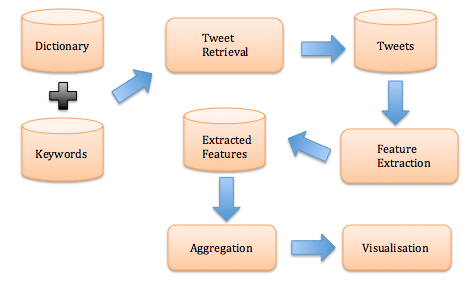
\includegraphics[width=10cm]{design}
\end{center}
\caption{General architecture of the system}
\label{fig:general}
\end{figure}

\subsection{Retrieving Tweets}
\label{sec:arc1}
The first stage involves retrieving tweets from Twitter. The design for this stage follows the same concepts for each of the use cases defined.
\subsection{Feature Extraction}
\label{sec:arc2}
\subsection{Visualisation}
\label{sec:arc3}